%!TEX root = ../../Master.tex
\section{Organisation}
\frnote{Her mangler lidt intro/ meta tekst}

Der er 4 store lystbådehavne i Aalborg by:
\begin{itemize}
    \item Marina Fjordpark
    \item Skudehavnen - lystbådehavnsafsnit
    \item Vestre Baadehavn - lystbådehavnsafsnit
    \item Nordre Baadehavn
\end{itemize}

I Aalborg er det kommunen der ejer alle havnene. ANF, en paraplyorganisation for sejlklubsforeninger i Aalborg/Nørresundby, får lov til at bruge disse havne i mod at havnene bliver vedligeholdt. Foreningerne i ANF kan så leje havnene af ANF. Der er typisk en bådklub pr. havn. Nogle havne benyttes også af mindre klubber som kajakklubber eller søspejdere.

\subsection{Aalborg/Nørresundby Fritidshavn}

ANF er en paraplyorganisation for følgende sejlklubber \cite{anf_havnereglement}.
\begin{itemize}
	\item Aalborg Sejlklub
	\item Fiskerklyngen
	\item Vestre Baadelaug
	\item Sejlklubben Limfjorden
	\item Nørresundby Sejlklub
\end{itemize}
 
ANF forestår forhandlinger på vegne af organisationens sejlklubber. En fælles brugsaftale af de fire havne, kan derved indgås med havneejer, Aalborg kommune.

ANF's indtægter består af bådpladsafgifter, som medlemsklubberne skal betale for brug af de tilknyttede havne \cite{anf_budget_2013}. ANF forpligter sig til vedligeholdelse af havnene tilknyttet foreningen, herunder hovedistandsættelser samt udføring af nyanlæg \cite{anf_brugsaftale_2012}.

\begin{figure}
  \centering
  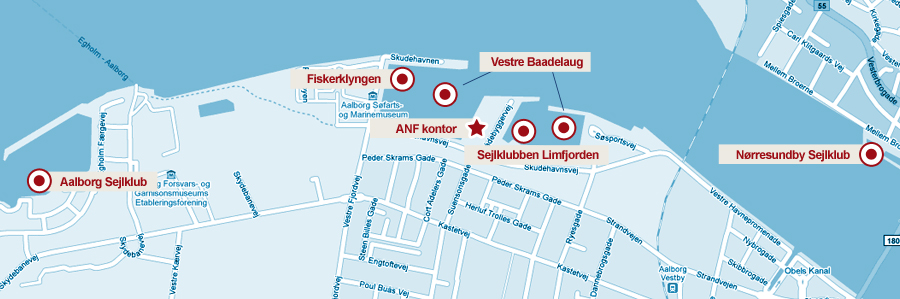
\includegraphics[width=\textwidth]{anf_overblik.jpg}
 	\caption{Overblik over medlemmerne af ANF} 	\label{fig:anf_overblik}
\end{figure}

\subsection{Bådklubber}
\frnote{vi skal måske havde et afsnit om plads fordeling}
Her vil vi se på de forskellige bådklubber der er med i ANF. Klubberne fordeler deres pladser ud til medlemmerne. I Vestre Baadelaug, en sejlkln, fordeles disse pladser hvert år ud til medlemmerne. Inden den nye pladsfordeling bliver lavet, er det være muligt at ønske en bestemt plads. Der er en masse menneskelige interesser der skal varetages når pladserne skal fordeles. Det er vigtigt for nogle mennesker hvor de ligger. Det er ikke muligt at få en permanent plads, kaseren sørge for at et medlem beholder sin plads når fordelingen bliver lavet. Medlemmerne betaler pr. kvadratmeter. Kvadratmeterne kan opgøres på forskellige måder, f.eks.\ som plads arealet eller som bådarealet. Et medlem kan kun have en bådplads, dog kan der opstå situationer hvor et medlem har mere end en båd, bl.a.\ i forbindelse med salg af en båd \cite{int_vb_sl}.

\subsubsection{Vestre Baadelaug}
Vestre Baadelaug har bådpladser i Vestre Bådehavn og Skudehavnen, som begge deles med Sejlklubben Limfjorden. Klubben har omkring 380 medlemmer \cite{int_vb_sl}. 

\subsection{Sejlkubben Limfjorden}
Sejlkubben Limfjorden har omkring 150 medlemmer \cite{int_vb_sl}. Klubbens medlemmer omfatter kun personer med sejlbåde. Klubben er medlem af Dansk Sejlunion (DS), som er et specialforbund under Dansk Idræts Forbund. DS optager klubber i alle former for sejlads, som medlemmer. DS har en kollektiv forsikring som medlemsklubberne automatisk er medlem af. 

\subsection{Aalborg Sejlklub}
Aalborg Sejlkulb er en Sejlklub, der hører til i havnen Marina Fjordparken.

\subsection{Nørresundby Sejlklub}
Nørresundby Sejlklub er tilknyttet Nørresundby havn. Klubben er medlem af Danske Tursejlere \cite{norresundby_sejlklub}.

\subsection{Regler og love}
Transportministeriet har i 2002 udgivet en bekendtgørelse om standardreglement for lystbådehavne \cite{standardreglement}. I denne er der regler om hvordan medlemmer samt gæster skal opføre sig når de befinder sig en havn. De enkelte havne skal udarbejde et individuelt ordensreglement, som beskriver hvilket område det gælder for, og hvilke særlige ordensregler der skal gælde på havnen. Derudover skal det referere til bekendtgørelsen.

I standardreglementet bliver der beskrevet hvordan ens fartøj skal fortøjes og hvordan der skal sejles i havne. Blandt andet står der at gæstende fartøjer skal melde deres ankomst til havnemyndigheden, og de skal flytte deres fartøj til en anden plads hvis havnemyndigheden siger det. Medlemmerne har også pligt til jævnligt at holde øje med sit fartøj, når det ligger i havnen. Fartøjet skal være forsvarligt fortøjret og tov skal fastgøres så de ikke klapper mod masten. I reglementet er der regler for optagning, reparation, brændstof og forskellige miljøbestemmelser.
